\documentclass{article}
\usepackage[T1]{fontenc}
\usepackage{lmodern}
\usepackage{graphicx}
\usepackage{amsmath,amssymb}
\usepackage[a4paper,margin=2cm]{geometry}
\usepackage[absolute,overlay]{textpos}
\setlength{\TPHorizModule}{1mm}
\setlength{\TPVertModule}{1mm}
\usepackage[indonesian]{babel}
\usepackage{hyperref}
\setlength{\emergencystretch}{2em}
% unit: Halaman 39

\begin{document}

% === Halaman 39 (llm) ===

\vspace{160.38mm}

\section*{Dekripsi}

% deskripsi: Potongan kode program C++ untuk implementasi proses dekripsi algoritma Rijndael (AES), mencakup definisi konstanta, fungsi decrypt\_rijndael, dan langkah-langkah seperti InvShiftRows, InvSubBytes, AddRoundKey, dan InvMixColumns.
% bbox normalisasi: [0.2900, 0.4000, 0.9100, 0.9400]
\begin{textblock*}{130.20mm}(60.90mm,118.80mm)
\noindent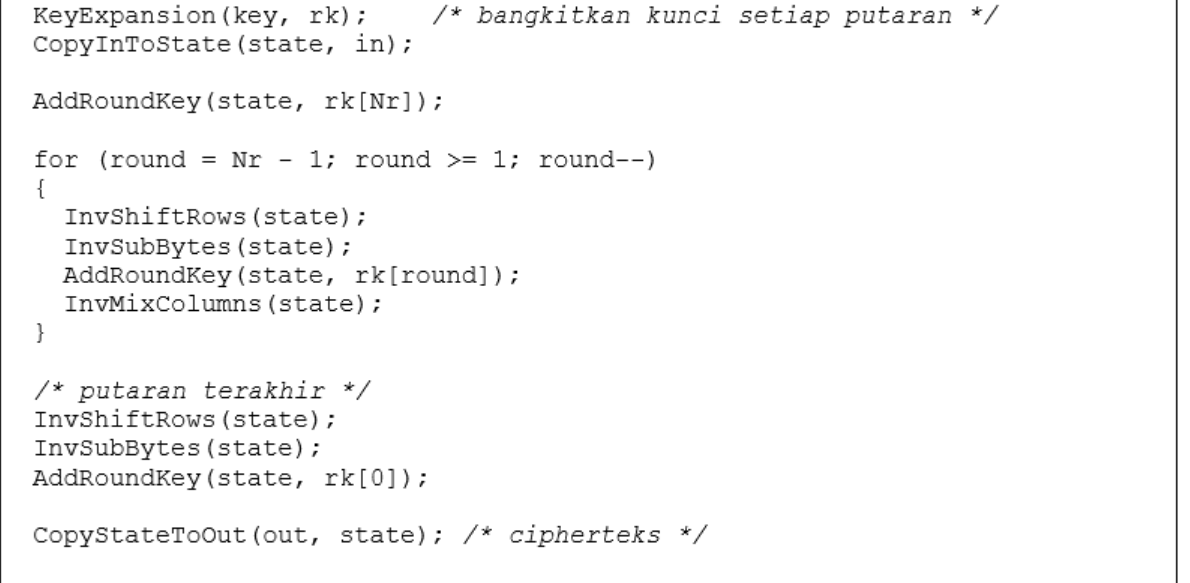
\includegraphics[width=130.20mm,height=160.38mm]{../../images/llm/page_039_img_01.png}%
\end{textblock*}

\end{document}
